%% LyX 2.2.1 created this file.  For more info, see http://www.lyx.org/.
\documentclass{article}\usepackage[]{graphicx}\usepackage[]{color}
%% maxwidth is the original width if it is less than linewidth
%% otherwise use linewidth (to make sure the graphics do not exceed the margin)
\makeatletter
\def\maxwidth{ %
  \ifdim\Gin@nat@width>\linewidth
    \linewidth
  \else
    \Gin@nat@width
  \fi
}
\makeatother

\definecolor{fgcolor}{rgb}{0.345, 0.345, 0.345}
\newcommand{\hlnum}[1]{\textcolor[rgb]{0.686,0.059,0.569}{#1}}%
\newcommand{\hlstr}[1]{\textcolor[rgb]{0.192,0.494,0.8}{#1}}%
\newcommand{\hlcom}[1]{\textcolor[rgb]{0.678,0.584,0.686}{\textit{#1}}}%
\newcommand{\hlopt}[1]{\textcolor[rgb]{0,0,0}{#1}}%
\newcommand{\hlstd}[1]{\textcolor[rgb]{0.345,0.345,0.345}{#1}}%
\newcommand{\hlkwa}[1]{\textcolor[rgb]{0.161,0.373,0.58}{\textbf{#1}}}%
\newcommand{\hlkwb}[1]{\textcolor[rgb]{0.69,0.353,0.396}{#1}}%
\newcommand{\hlkwc}[1]{\textcolor[rgb]{0.333,0.667,0.333}{#1}}%
\newcommand{\hlkwd}[1]{\textcolor[rgb]{0.737,0.353,0.396}{\textbf{#1}}}%

\usepackage{framed}
\makeatletter
\newenvironment{kframe}{%
 \def\at@end@of@kframe{}%
 \ifinner\ifhmode%
  \def\at@end@of@kframe{\end{minipage}}%
  \begin{minipage}{\columnwidth}%
 \fi\fi%
 \def\FrameCommand##1{\hskip\@totalleftmargin \hskip-\fboxsep
 \colorbox{shadecolor}{##1}\hskip-\fboxsep
     % There is no \\@totalrightmargin, so:
     \hskip-\linewidth \hskip-\@totalleftmargin \hskip\columnwidth}%
 \MakeFramed {\advance\hsize-\width
   \@totalleftmargin\z@ \linewidth\hsize
   \@setminipage}}%
 {\par\unskip\endMakeFramed%
 \at@end@of@kframe}
\makeatother

\definecolor{shadecolor}{rgb}{.97, .97, .97}
\definecolor{messagecolor}{rgb}{0, 0, 0}
\definecolor{warningcolor}{rgb}{1, 0, 1}
\definecolor{errorcolor}{rgb}{1, 0, 0}
\newenvironment{knitrout}{}{} % an empty environment to be redefined in TeX

\usepackage{alltt}
\usepackage[sc]{mathpazo}
\usepackage[T1]{fontenc}
\usepackage{geometry}
\geometry{verbose,tmargin=2.5cm,bmargin=2.5cm,lmargin=2.5cm,rmargin=2.5cm}
\setcounter{secnumdepth}{2}
\setcounter{tocdepth}{2}
\usepackage{url}
\usepackage[unicode=true,pdfusetitle,
 bookmarks=true,bookmarksnumbered=true,bookmarksopen=true,bookmarksopenlevel=2,
 breaklinks=false,pdfborder={0 0 1},backref=false,colorlinks=false]
 {hyperref}
\hypersetup{
 pdfstartview={XYZ null null 1}}
\usepackage{breakurl}
\IfFileExists{upquote.sty}{\usepackage{upquote}}{}
\begin{document}


\title{Linear and logistic regression}

\maketitle

We can review linear regression using a dataset of Grandfather clocks. We can look at simple linear regression and multiple linear regression. We can also review parameter interpretations, including for interactive terms.

\begin{knitrout}
\definecolor{shadecolor}{rgb}{0.969, 0.969, 0.969}\color{fgcolor}\begin{kframe}
\begin{alltt}
\hlcom{# Read in the clocks dataset}
\hlstd{clocksDat} \hlkwb{=} \hlkwd{read.csv}\hlstd{(}\hlstr{"clocks.csv"}\hlstd{)}
\hlstd{clocksDat}
\end{alltt}
\begin{verbatim}
##    Age Bidders Price
## 1  127      13  1235
## 2  115      12  1080
## 3  127       7   845
## 4  150       9  1522
## 5  156       6  1047
## 6  182      11  1979
## 7  156      12  1822
## 8  132      10  1253
## 9  137       9  1297
## 10 113       9   946
## 11 137      15  1713
## 12 117      11  1024
## 13 137       8  1147
## 14 153       6  1092
## 15 117      13  1152
## 16 126      10  1336
## 17 170      14  2131
## 18 182       8  1550
## 19 162      11  1884
## 20 184      10  2041
## 21 143       6   854
## 22 159       9  1483
## 23 108      14  1055
## 24 175       8  1545
## 25 108       6   729
## 26 179       9  1792
## 27 111      15  1175
## 28 187       8  1593
## 29 111       7   785
## 30 115       7   744
## 31 194       5  1356
## 32 168       7  1262
\end{verbatim}
\begin{alltt}
\hlkwd{plot}\hlstd{(clocksDat,}\hlkwc{pch}\hlstd{=}\hlnum{16}\hlstd{)}
\end{alltt}
\end{kframe}
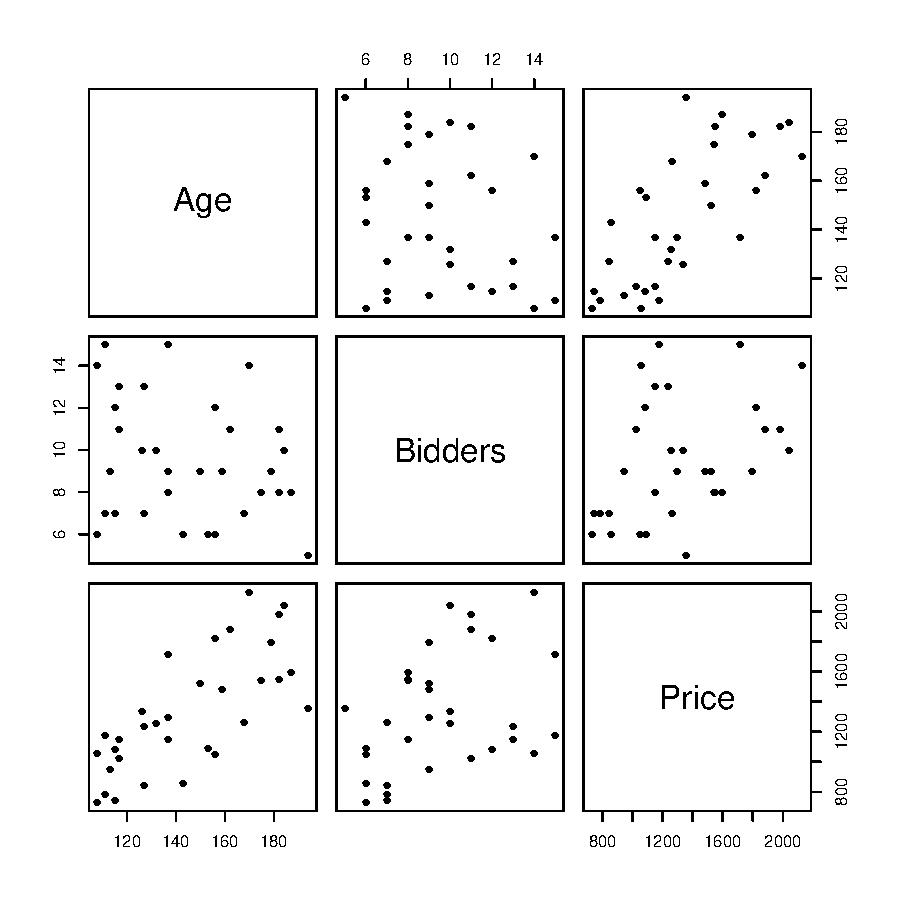
\includegraphics[width=.6\linewidth]{figure/unnamed-chunk-1-1} 

\end{knitrout}

\section{Simple linear regression}

We can first perform simple linear regression with one quantitative explanatory variable - age.

\begin{knitrout}
\definecolor{shadecolor}{rgb}{0.969, 0.969, 0.969}\color{fgcolor}\begin{kframe}
\begin{alltt}
\hlstd{clocksLinAge} \hlkwb{=} \hlkwd{lm}\hlstd{(Price} \hlopt{~} \hlstd{Age,} \hlkwc{data}\hlstd{=clocksDat)}
\hlkwd{summary}\hlstd{(clocksLinAge)}
\end{alltt}
\begin{verbatim}
## 
## Call:
## lm(formula = Price ~ Age, data = clocksDat)
## 
## Residuals:
##     Min      1Q  Median      3Q     Max 
## -485.29 -192.66   30.75  157.21  541.21 
## 
## Coefficients:
##             Estimate Std. Error t value Pr(>|t|)    
## (Intercept)  -191.66     263.89  -0.726    0.473    
## Age            10.48       1.79   5.854  2.1e-06 ***
## ---
## Signif. codes:  
## 0 '***' 0.001 '**' 0.01 '*' 0.05 '.' 0.1 ' ' 1
## 
## Residual standard error: 273 on 30 degrees of freedom
## Multiple R-squared:  0.5332,	Adjusted R-squared:  0.5177 
## F-statistic: 34.27 on 1 and 30 DF,  p-value: 2.096e-06
\end{verbatim}
\end{kframe}
\end{knitrout}

\newpage

We can visualize what this best-fit line appears like.

\begin{knitrout}
\definecolor{shadecolor}{rgb}{0.969, 0.969, 0.969}\color{fgcolor}\begin{kframe}
\begin{alltt}
\hlstd{intercept} \hlkwb{=} \hlkwd{coef}\hlstd{(clocksLinAge)[}\hlstr{"(Intercept)"}\hlstd{]}
\hlstd{age} \hlkwb{=} \hlkwd{coef}\hlstd{(clocksLinAge)[}\hlstr{"Age"}\hlstd{]}
\hlstd{q} \hlkwb{=} \hlkwd{qplot}\hlstd{(clocksDat}\hlopt{$}\hlstd{Age,clocksDat}\hlopt{$}\hlstd{Price)}
\hlstd{q} \hlkwb{=} \hlstd{q} \hlopt{+} \hlkwd{geom_abline}\hlstd{(}\hlkwc{intercept} \hlstd{= intercept,} \hlkwc{slope} \hlstd{= age)} \hlopt{+} \hlkwd{xlim}\hlstd{(}\hlopt{-}\hlnum{10}\hlstd{,}\hlnum{200}\hlstd{)} \hlopt{+} \hlkwd{ylim}\hlstd{(}\hlopt{-}\hlnum{1000}\hlstd{,}\hlnum{2200}\hlstd{)}
\hlstd{q} \hlopt{+} \hlkwd{xlab}\hlstd{(}\hlstr{"Clock age"}\hlstd{)} \hlopt{+} \hlkwd{ylab}\hlstd{(}\hlstr{"Clock price"}\hlstd{)}
\end{alltt}
\end{kframe}
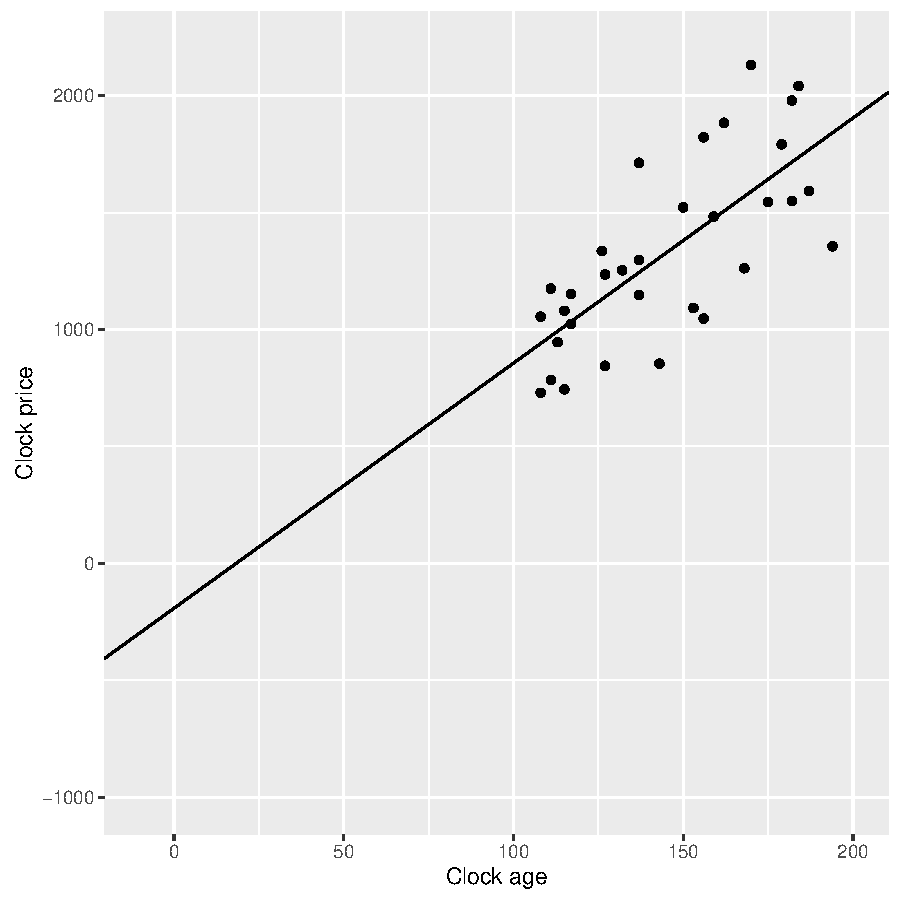
\includegraphics[width=.6\linewidth]{figure/unnamed-chunk-3-1} 

\end{knitrout}

\vspace{15mm}

\textbf{1) What is the interpretation for the intercept?}

\vspace{20mm}

\textbf{2) What is the interpretation for the slope?}

\vspace{20mm}

\textbf{3) How much would we predict a 175 year old clock would cost?}

\vspace{20mm}

\newpage

\section{Multiple linear regression - no interaction terms}

Now, we can perform multiple linear regression with two quantitative variables - age and number of bidders.

\begin{knitrout}
\definecolor{shadecolor}{rgb}{0.969, 0.969, 0.969}\color{fgcolor}\begin{kframe}
\begin{alltt}
\hlstd{clocksLinAgeBid} \hlkwb{=} \hlkwd{lm}\hlstd{(Price} \hlopt{~} \hlstd{Age} \hlopt{+} \hlstd{Bidders,} \hlkwc{data}\hlstd{=clocksDat)}
\hlkwd{summary}\hlstd{(clocksLinAgeBid)}
\end{alltt}
\begin{verbatim}
## 
## Call:
## lm(formula = Price ~ Age + Bidders, data = clocksDat)
## 
## Residuals:
##    Min     1Q Median     3Q    Max 
## -207.2 -117.8   16.5  102.7  213.5 
## 
## Coefficients:
##               Estimate Std. Error t value Pr(>|t|)    
## (Intercept) -1336.7221   173.3561  -7.711 1.67e-08 ***
## Age            12.7362     0.9024  14.114 1.60e-14 ***
## Bidders        85.8151     8.7058   9.857 9.14e-11 ***
## ---
## Signif. codes:  
## 0 '***' 0.001 '**' 0.01 '*' 0.05 '.' 0.1 ' ' 1
## 
## Residual standard error: 133.1 on 29 degrees of freedom
## Multiple R-squared:  0.8927,	Adjusted R-squared:  0.8853 
## F-statistic: 120.7 on 2 and 29 DF,  p-value: 8.769e-15
\end{verbatim}
\end{kframe}
\end{knitrout}

\vspace{5mm}

\textbf{4) What is the interpretation for the intercept?}

\vspace{20mm}

\textbf{5) What is the interpretation for the age slope?}

\vspace{20mm}

\textbf{6) What is the interpretation for the bidders slope?}

\vspace{20mm}

\textbf{7) How much would we predict a 194 year old clock would cost if there are 5 bidders?}

\newpage

\section{Multiple linear regression - with interaction term}

When we did not use an interaction term above, we assumed that the price change due to a change in age would not be affected by the number of bidders. Likewise, we also assumed that the price change due to a change in the number of bidders would not be affected by the age.

\vspace{5mm}

\fbox{\includegraphics[width=0.5\textwidth]{noint.png}}

\vspace{5mm}

\noindent However, it could be the case that the independent variables do have an interactive effect. In this case, the linear relationship between price and age would have a different slope coefficient depending on the number of bidders. Likewise, the linear relationship between price and number of bidders would have a different slope coefficient depending on the age.

\vspace{5mm}

\fbox{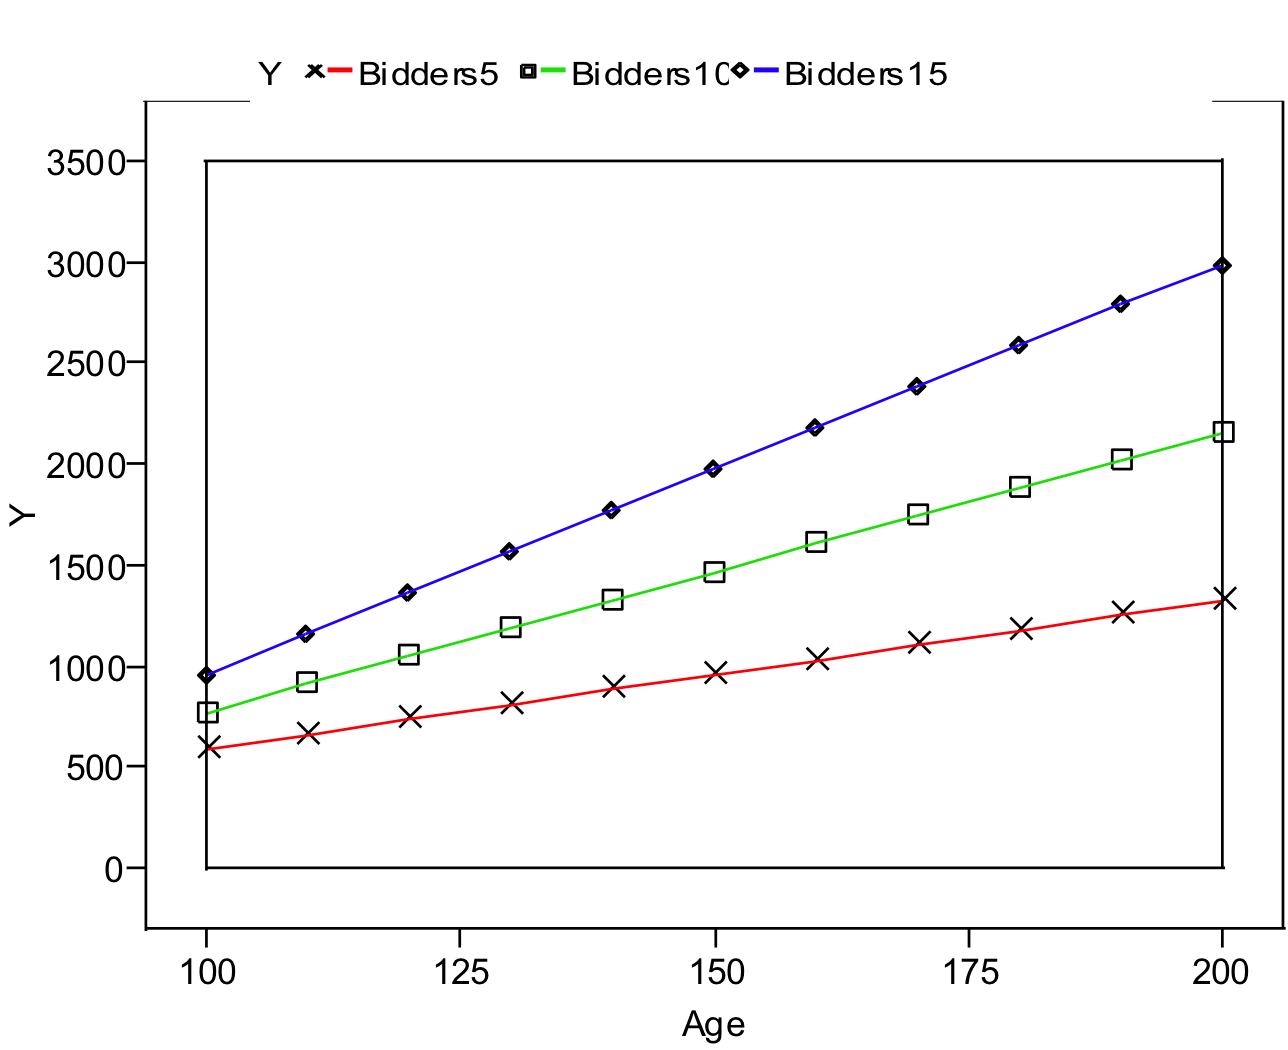
\includegraphics[width=0.5\textwidth]{int.png}}

\vspace{5mm}

\noindent As a result, at this stage, we might want to determine if the two independent variables have an interactive effect.

\begin{knitrout}
\definecolor{shadecolor}{rgb}{0.969, 0.969, 0.969}\color{fgcolor}\begin{kframe}
\begin{alltt}
\hlstd{clocksLinAgeBidInt} \hlkwb{=} \hlkwd{lm}\hlstd{(Price} \hlopt{~} \hlstd{Age} \hlopt{+} \hlstd{Bidders} \hlopt{+} \hlstd{Age}\hlopt{*}\hlstd{Bidders,} \hlkwc{data}\hlstd{=clocksDat)}
\hlkwd{summary}\hlstd{(clocksLinAgeBidInt)}
\end{alltt}
\begin{verbatim}
## 
## Call:
## lm(formula = Price ~ Age + Bidders + Age * Bidders, data = clocksDat)
## 
## Residuals:
##      Min       1Q   Median       3Q      Max 
## -146.772  -70.985    2.108   47.535  201.959 
## 
## Coefficients:
##             Estimate Std. Error t value Pr(>|t|)    
## (Intercept) 322.7544   293.3251   1.100  0.28056    
## Age           0.8733     2.0197   0.432  0.66877    
## Bidders     -93.4099    29.7077  -3.144  0.00392 ** 
## Age:Bidders   1.2979     0.2110   6.150 1.22e-06 ***
## ---
## Signif. codes:  
## 0 '***' 0.001 '**' 0.01 '*' 0.05 '.' 0.1 ' ' 1
## 
## Residual standard error: 88.37 on 28 degrees of freedom
## Multiple R-squared:  0.9544,	Adjusted R-squared:  0.9495 
## F-statistic: 195.2 on 3 and 28 DF,  p-value: < 2.2e-16
\end{verbatim}
\end{kframe}
\end{knitrout}

\vspace{5mm}

\textbf{8) What is the interpretation for the age slope?}

\vspace{20mm}

\textbf{9) What is the interpretation for the number of bidders slope?}

\vspace{20mm}

\textbf{10) How much would we predict a 194 year old clock would cost if there are 5 bidders?}

\vspace{20mm}

\textbf{11) Which model would you use? Simple linear regression? Multiple linear regression without interaction term? Or, multiple lienar regression with interaction term?}

\newpage

\section{Binomial Logistic Regression}

We can use a lobster survival dataset to perform binomial logistic regression.

\begin{knitrout}
\definecolor{shadecolor}{rgb}{0.969, 0.969, 0.969}\color{fgcolor}\begin{kframe}
\begin{alltt}
\hlstd{lobsterDat} \hlkwb{=} \hlkwd{read.csv}\hlstd{(}\hlstr{"lobster.csv"}\hlstd{)}
\hlkwd{colnames}\hlstd{(lobsterDat)} \hlkwb{=} \hlkwd{c}\hlstd{(}\hlstr{"carpaceLength"}\hlstd{,}\hlstr{"survive"}\hlstd{)}
\hlkwd{dim}\hlstd{(lobsterDat)}
\end{alltt}
\begin{verbatim}
## [1] 158   2
\end{verbatim}
\begin{alltt}
\hlkwd{head}\hlstd{(lobsterDat)}
\end{alltt}
\begin{verbatim}
##   carpaceLength survive
## 1            27       0
## 2            27       0
## 3            27       0
## 4            27       0
## 5            30       0
## 6            30       0
\end{verbatim}
\end{kframe}
\end{knitrout}

\begin{knitrout}
\definecolor{shadecolor}{rgb}{0.969, 0.969, 0.969}\color{fgcolor}\begin{kframe}
\begin{alltt}
\hlstd{lobsterLogit} \hlkwb{<-} \hlkwd{glm}\hlstd{(survive} \hlopt{~} \hlstd{carpaceLength,} \hlkwc{data} \hlstd{= lobsterDat,} \hlkwc{family} \hlstd{=} \hlstr{"binomial"}\hlstd{)}
\hlstd{lobsterLogit}
\end{alltt}
\begin{verbatim}
## 
## Call:  glm(formula = survive ~ carpaceLength, family = "binomial", data = lobsterDat)
## 
## Coefficients:
##   (Intercept)  carpaceLength  
##       -7.8506         0.1948  
## 
## Degrees of Freedom: 157 Total (i.e. Null);  156 Residual
## Null Deviance:	    219 
## Residual Deviance: 172.7 	AIC: 176.7
\end{verbatim}
\end{kframe}
\end{knitrout}

Now that we have the coefficient estimations, we can plot the logistic function of the data.

\begin{knitrout}
\definecolor{shadecolor}{rgb}{0.969, 0.969, 0.969}\color{fgcolor}\begin{kframe}
\begin{alltt}
\hlstd{lobsterIntercept} \hlkwb{=} \hlkwd{coef}\hlstd{(lobsterLogit)[}\hlstr{"(Intercept)"}\hlstd{]}
\hlstd{lobsterCarpaceLength} \hlkwb{=} \hlkwd{coef}\hlstd{(lobsterLogit)[}\hlstr{"carpaceLength"}\hlstd{]}

\hlstd{carpaceLengths} \hlkwb{=} \hlkwd{seq}\hlstd{(}\hlnum{0}\hlstd{,}\hlnum{60}\hlstd{,}\hlnum{0.1}\hlstd{)}
\hlstd{survive} \hlkwb{=} \hlnum{1}\hlopt{/}\hlstd{(}\hlnum{1}\hlopt{+}\hlkwd{exp}\hlstd{(}\hlopt{-}\hlstd{(lobsterIntercept}\hlopt{+}\hlstd{lobsterCarpaceLength}\hlopt{*}\hlstd{carpaceLengths)))}
\hlstd{q} \hlkwb{=} \hlkwd{qplot}\hlstd{(carpaceLengths,survive)}
\hlstd{q} \hlkwb{=} \hlstd{q} \hlopt{+} \hlkwd{theme}\hlstd{(}\hlkwc{axis.text}\hlstd{=}\hlkwd{element_text}\hlstd{(}\hlkwc{size}\hlstd{=}\hlnum{14}\hlstd{),} \hlkwc{axis.title}\hlstd{=}\hlkwd{element_text}\hlstd{(}\hlkwc{size}\hlstd{=}\hlnum{14}\hlstd{))}
\hlstd{q}
\end{alltt}
\end{kframe}
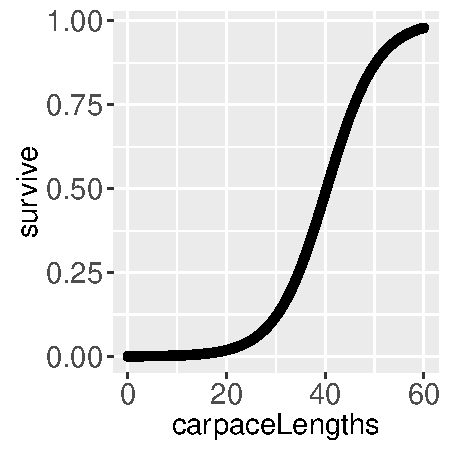
\includegraphics[width=.3\linewidth]{figure/unnamed-chunk-8-1} 

\end{knitrout}

\vspace{5mm}

\textbf{12) What is the probability of surviving if carpaceLength is 30mm?}

\vspace{20mm}

\textbf{13) What is the probability of surviving if carpaceLength is 31mm?}

\vspace{20mm}

\textbf{14) What is the probability of surviving if carpaceLength is 55mm?}

\vspace{20mm}

\textbf{15) What are the odds of survival if carpaceLength is 30mm?}

\vspace{20mm}

\textbf{16) What are the odds of survival if carpaceLength is 31mm?}

\vspace{20mm}

\textbf{17) What is the odds ratio?}

\vspace{20mm}

\textbf{18) What is the interpretation of the odds ratio?}

\newpage

\section{Multinomial Logistic Regression}

We can use a dataset regarding survival in the Titanic tragedy to perform multinomial logistic regression. This dataset was taken from the data science education and competition website Kaggle (\url{https://www.kaggle.com/}).

\begin{knitrout}
\definecolor{shadecolor}{rgb}{0.969, 0.969, 0.969}\color{fgcolor}\begin{kframe}
\begin{alltt}
\hlstd{titanicDat} \hlkwb{=} \hlkwd{read.csv}\hlstd{(}\hlstr{'titanic.csv'}\hlstd{,}\hlkwc{header}\hlstd{=T,}\hlkwc{na.strings}\hlstd{=}\hlkwd{c}\hlstd{(}\hlstr{""}\hlstd{))}
\hlkwd{dim}\hlstd{(titanicDat)}
\end{alltt}
\begin{verbatim}
## [1] 891  12
\end{verbatim}
\begin{alltt}
\hlkwd{head}\hlstd{(titanicDat)}
\end{alltt}
\begin{verbatim}
##   PassengerId Survived Pclass
## 1           1        0      3
## 2           2        1      1
## 3           3        1      3
## 4           4        1      1
## 5           5        0      3
## 6           6        0      3
##                                                  Name
## 1                             Braund, Mr. Owen Harris
## 2 Cumings, Mrs. John Bradley (Florence Briggs Thayer)
## 3                              Heikkinen, Miss. Laina
## 4        Futrelle, Mrs. Jacques Heath (Lily May Peel)
## 5                            Allen, Mr. William Henry
## 6                                    Moran, Mr. James
##      Sex Age SibSp Parch           Ticket    Fare Cabin
## 1   male  22     1     0        A/5 21171  7.2500  <NA>
## 2 female  38     1     0         PC 17599 71.2833   C85
## 3 female  26     0     0 STON/O2. 3101282  7.9250  <NA>
## 4 female  35     1     0           113803 53.1000  C123
## 5   male  35     0     0           373450  8.0500  <NA>
## 6   male  NA     0     0           330877  8.4583  <NA>
##   Embarked
## 1        S
## 2        C
## 3        S
## 4        S
## 5        S
## 6        Q
\end{verbatim}
\end{kframe}
\end{knitrout}

We examine missing data as a preprocessing step.

\begin{knitrout}
\definecolor{shadecolor}{rgb}{0.969, 0.969, 0.969}\color{fgcolor}\begin{kframe}
\begin{alltt}
\hlkwd{sapply}\hlstd{(titanicDat,}\hlkwa{function}\hlstd{(}\hlkwc{x}\hlstd{)} \hlkwd{sum}\hlstd{(}\hlkwd{is.na}\hlstd{(x)))}
\end{alltt}
\begin{verbatim}
## PassengerId    Survived      Pclass        Name         Sex 
##           0           0           0           0           0 
##         Age       SibSp       Parch      Ticket        Fare 
##         177           0           0           0           0 
##       Cabin    Embarked 
##         687           2
\end{verbatim}
\begin{alltt}
\hlcom{# R package to visualize missing data information}
\hlkwd{library}\hlstd{(Amelia)}
\hlkwd{missmap}\hlstd{(titanicDat,} \hlkwc{main} \hlstd{=} \hlstr{"Missing values vs observed"}\hlstd{)}
\end{alltt}
\end{kframe}
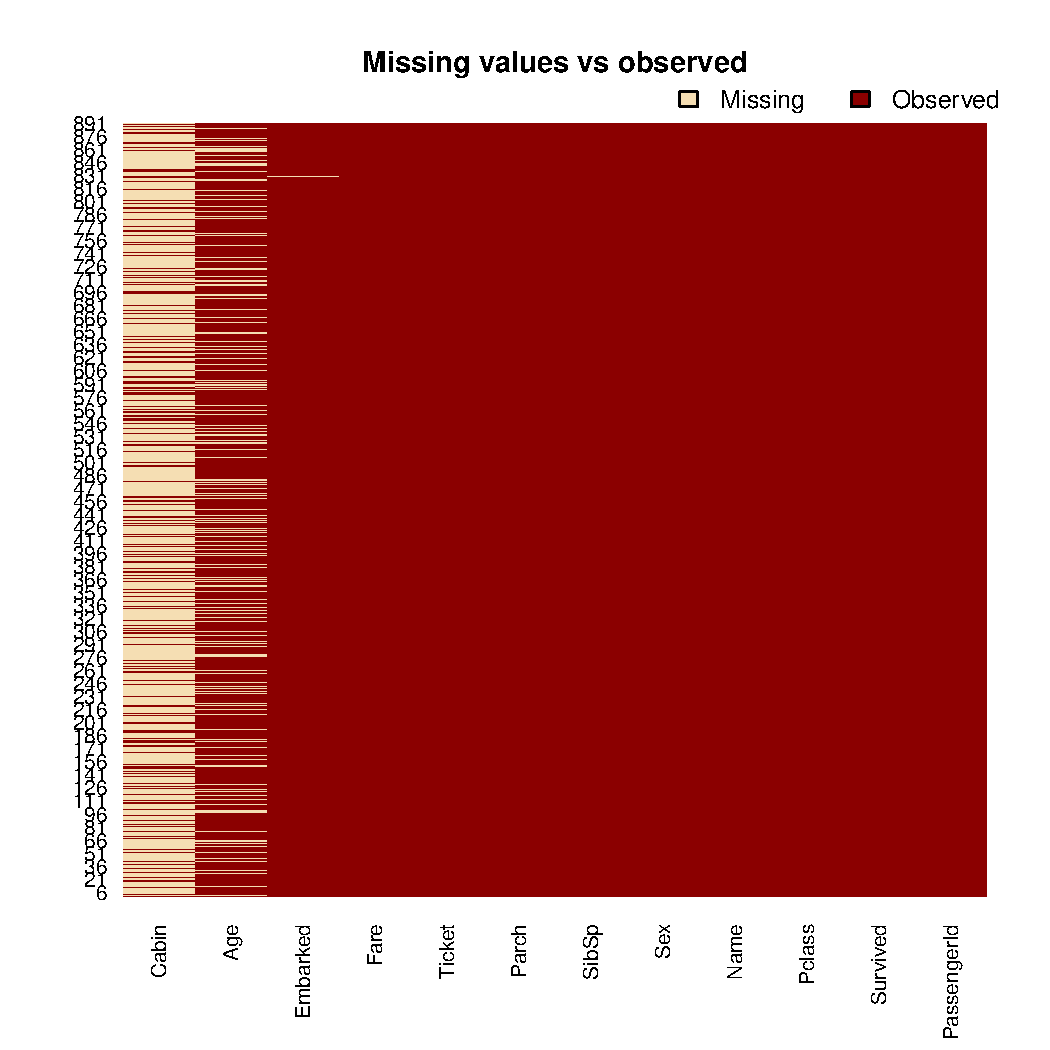
\includegraphics[width=.7\linewidth]{figure/unnamed-chunk-10-1} 

\end{knitrout}

We remove the columns for PassengerID, Name, Ticket, and Cabin (since it is missing so many values).

\begin{knitrout}
\definecolor{shadecolor}{rgb}{0.969, 0.969, 0.969}\color{fgcolor}\begin{kframe}
\begin{alltt}
\hlstd{titanicDat} \hlkwb{<-} \hlkwd{subset}\hlstd{(titanicDat,}\hlkwc{select}\hlstd{=}\hlkwd{c}\hlstd{(}\hlnum{2}\hlstd{,}\hlnum{3}\hlstd{,}\hlnum{5}\hlstd{,}\hlnum{6}\hlstd{,}\hlnum{7}\hlstd{,}\hlnum{8}\hlstd{,}\hlnum{10}\hlstd{,}\hlnum{12}\hlstd{))}
\end{alltt}
\end{kframe}
\end{knitrout}

There are many values missing from Age. We replace the missing values with the mean age of the known values (which was ~29.7).

\begin{knitrout}
\definecolor{shadecolor}{rgb}{0.969, 0.969, 0.969}\color{fgcolor}\begin{kframe}
\begin{alltt}
\hlstd{titanicDat}\hlopt{$}\hlstd{Age[}\hlkwd{is.na}\hlstd{(titanicDat}\hlopt{$}\hlstd{Age)]} \hlkwb{<-} \hlkwd{mean}\hlstd{(titanicDat}\hlopt{$}\hlstd{Age,}\hlkwc{na.rm}\hlstd{=T)}
\end{alltt}
\end{kframe}
\end{knitrout}

There are two row with missing values, so we remove them as well.

\begin{knitrout}
\definecolor{shadecolor}{rgb}{0.969, 0.969, 0.969}\color{fgcolor}\begin{kframe}
\begin{alltt}
\hlstd{titanicDat} \hlkwb{<-} \hlstd{titanicDat[}\hlopt{!}\hlkwd{is.na}\hlstd{(titanicDat}\hlopt{$}\hlstd{Embarked),]}
\hlkwd{rownames}\hlstd{(titanicDat)} \hlkwb{<-} \hlkwa{NULL}
\end{alltt}
\end{kframe}
\end{knitrout}

We can verify that we know what the indicators are for the variable Sex.

\begin{knitrout}
\definecolor{shadecolor}{rgb}{0.969, 0.969, 0.969}\color{fgcolor}\begin{kframe}
\begin{alltt}
\hlkwd{contrasts}\hlstd{(titanicDat}\hlopt{$}\hlstd{Sex)}
\end{alltt}
\begin{verbatim}
##        male
## female    0
## male      1
\end{verbatim}
\end{kframe}
\end{knitrout}

We now have 889 rows of clean data. We can split these data into a training and test set as follows:

\begin{knitrout}
\definecolor{shadecolor}{rgb}{0.969, 0.969, 0.969}\color{fgcolor}\begin{kframe}
\begin{alltt}
\hlstd{trainDat} \hlkwb{<-} \hlstd{titanicDat[}\hlnum{1}\hlopt{:}\hlnum{800}\hlstd{,]}
\hlstd{testDat} \hlkwb{<-} \hlstd{titanicDat[}\hlnum{801}\hlopt{:}\hlnum{889}\hlstd{,]}
\end{alltt}
\end{kframe}
\end{knitrout}

We can run a binomial logistic regression with the only explanatory variable being sex.

\begin{knitrout}
\definecolor{shadecolor}{rgb}{0.969, 0.969, 0.969}\color{fgcolor}\begin{kframe}
\begin{alltt}
\hlstd{titanicLogit} \hlkwb{<-} \hlkwd{glm}\hlstd{(Survived} \hlopt{~} \hlstd{Sex,} \hlkwc{data} \hlstd{= titanicDat,} \hlkwc{family} \hlstd{=} \hlstr{"binomial"}\hlstd{)}
\hlstd{titanicLogit}
\end{alltt}
\begin{verbatim}
## 
## Call:  glm(formula = Survived ~ Sex, family = "binomial", data = titanicDat)
## 
## Coefficients:
## (Intercept)      Sexmale  
##       1.048       -2.505  
## 
## Degrees of Freedom: 888 Total (i.e. Null);  887 Residual
## Null Deviance:	    1183 
## Residual Deviance: 916.6 	AIC: 920.6
\end{verbatim}
\end{kframe}
\end{knitrout}

\vspace{5mm}

\textbf{19) What is the probability of surviving if male?}

\vspace{20mm}

\textbf{20) What is the probability of surviving if female?}

\vspace{20mm}

\textbf{21) What are the odds of surviving if male?}

\vspace{20mm}

\textbf{22) What are the odds of surviving if female?}

\vspace{20mm}

\textbf{23) What is the odds ratio?}

\vspace{20mm}

\textbf{24) What is the interpretation of the odds ratio?}

\newpage

Now, we can consider more than one explanatory variable. Let's consider all explanatory variables that remain in the cleaned data.

\begin{knitrout}
\definecolor{shadecolor}{rgb}{0.969, 0.969, 0.969}\color{fgcolor}\begin{kframe}
\begin{alltt}
\hlstd{titanicLogitFull} \hlkwb{<-} \hlkwd{glm}\hlstd{(Survived} \hlopt{~} \hlstd{.,} \hlkwc{data} \hlstd{= titanicDat,} \hlkwc{family} \hlstd{=} \hlstr{"binomial"}\hlstd{)}
\hlkwd{summary}\hlstd{(titanicLogitFull)}
\end{alltt}
\begin{verbatim}
## 
## Call:
## glm(formula = Survived ~ ., family = "binomial", data = titanicDat)
## 
## Deviance Residuals: 
##     Min       1Q   Median       3Q      Max  
## -2.6446  -0.5907  -0.4230   0.6220   2.4431  
## 
## Coefficients:
##              Estimate Std. Error z value Pr(>|z|)    
## (Intercept)  5.285188   0.564778   9.358  < 2e-16 ***
## Pclass      -1.100058   0.143529  -7.664 1.80e-14 ***
## Sexmale     -2.718695   0.200783 -13.540  < 2e-16 ***
## Age         -0.039901   0.007854  -5.080 3.77e-07 ***
## SibSp       -0.325777   0.109384  -2.978   0.0029 ** 
## Parch       -0.092602   0.118708  -0.780   0.4353    
## Fare         0.001918   0.002376   0.807   0.4194    
## EmbarkedQ   -0.034076   0.381936  -0.089   0.9289    
## EmbarkedS   -0.418817   0.236794  -1.769   0.0769 .  
## ---
## Signif. codes:  
## 0 '***' 0.001 '**' 0.01 '*' 0.05 '.' 0.1 ' ' 1
## 
## (Dispersion parameter for binomial family taken to be 1)
## 
##     Null deviance: 1182.82  on 888  degrees of freedom
## Residual deviance:  784.19  on 880  degrees of freedom
## AIC: 802.19
## 
## Number of Fisher Scoring iterations: 5
\end{verbatim}
\end{kframe}
\end{knitrout}

\vspace{5mm}

\textbf{25) What is the interpretation of the odds ratio for age?}

\vspace{20mm}

\textbf{26) What is the interpretation of the odds ratio for class?}

\vspace{20mm}

We can use ANOVA to examine the difference between the null deviance (model with only intercept) and the residual deviance. The table shows that the deviance drops when adding each variable one at a time. However, the p-values show that only Pclass, Sex, Age, and Sibsp show a significant drop in residual deviance.

\begin{knitrout}
\definecolor{shadecolor}{rgb}{0.969, 0.969, 0.969}\color{fgcolor}\begin{kframe}
\begin{alltt}
\hlkwd{anova}\hlstd{(titanicLogitFull,} \hlkwc{test}\hlstd{=}\hlstr{"Chisq"}\hlstd{)}
\end{alltt}
\begin{verbatim}
## Analysis of Deviance Table
## 
## Model: binomial, link: logit
## 
## Response: Survived
## 
## Terms added sequentially (first to last)
## 
## 
##          Df Deviance Resid. Df Resid. Dev  Pr(>Chi)    
## NULL                       888    1182.82              
## Pclass    1  100.179       887    1082.64 < 2.2e-16 ***
## Sex       1  255.814       886     826.82 < 2.2e-16 ***
## Age       1   22.101       885     804.72 2.587e-06 ***
## SibSp     1   14.423       884     790.30  0.000146 ***
## Parch     1    0.497       883     789.80  0.480798    
## Fare      1    1.578       882     788.22  0.209046    
## Embarked  2    4.036       880     784.19  0.132904    
## ---
## Signif. codes:  
## 0 '***' 0.001 '**' 0.01 '*' 0.05 '.' 0.1 ' ' 1
\end{verbatim}
\end{kframe}
\end{knitrout}

\vspace{5mm}

We can assess how well our full model fits the testing data now! We can obtain probabilities in the form of P(Y=1|X). We can use a decision boundary of 0.5. In other words, if P(Y=1|X) > 0.5, then Y=1. Otherwise, Y=0. We then compare this to the actual values of survival being 1 (Survived) or 0 (Died).

\begin{knitrout}
\definecolor{shadecolor}{rgb}{0.969, 0.969, 0.969}\color{fgcolor}\begin{kframe}
\begin{alltt}
\hlstd{fitRes} \hlkwb{=} \hlkwd{predict}\hlstd{(titanicLogitFull,}\hlkwc{newdata}\hlstd{=}\hlkwd{subset}\hlstd{(testDat,}\hlkwc{select}\hlstd{=}\hlkwd{c}\hlstd{(}\hlnum{2}\hlstd{,}\hlnum{3}\hlstd{,}\hlnum{4}\hlstd{,}\hlnum{5}\hlstd{,}\hlnum{6}\hlstd{,}\hlnum{7}\hlstd{,}\hlnum{8}\hlstd{)),}\hlkwc{type}\hlstd{=}\hlstr{'response'}\hlstd{)}
\hlstd{fitRes} \hlkwb{=} \hlkwd{ifelse}\hlstd{(fitRes} \hlopt{>} \hlnum{0.5}\hlstd{,}\hlnum{1}\hlstd{,}\hlnum{0}\hlstd{)}
\hlstd{misClasificError} \hlkwb{=} \hlkwd{mean}\hlstd{(fitRes} \hlopt{!=} \hlstd{testDat}\hlopt{$}\hlstd{Survived)}
\hlkwd{print}\hlstd{(}\hlkwd{paste}\hlstd{(}\hlstr{'Accuracy'}\hlstd{,}\hlnum{1}\hlopt{-}\hlstd{misClasificError))}
\end{alltt}
\begin{verbatim}
## [1] "Accuracy 0.853932584269663"
\end{verbatim}
\end{kframe}
\end{knitrout}

\end{document}
